\documentclass[main.tex]{subfiles}
\begin{document}
\subsection{平衡态的稳定性简介}
我们知道,由热力学第二定律,以温度、压强和组成$\left(T,p,\left\{n_i\right\}\right)$作为状态参数的体系,任何可能发生的变动都使其特性函数——吉布斯自由能——的变化小于零。那么,假定体系被实验控制在$\left(T^\circ,p^\circ,\left\{n_i^\circ\right\}\right)$下,考虑体系由此状态出发至任一微小变化后的状态$\left(T^\circ+\Delta T,p^\circ+\Delta p,\left\{n_i^\circ+\Delta n_i\right\}\right)$造成的吉布斯自由能变$\Delta^\circ G$,必须总小于零——否则体系在不加控制的情况下就会自发离开当前状态点$\left(T^\circ,p^\circ,\left\{n_i^\circ\right\}\right)$往某一个吉布斯自由能值更小方向变化。实验上,我们碰到的问题常常并不是把所有状态参量都控制住的。若在某实验中,我们只控制体系的部分状态量恒定,任由体系自发变化剩余的状态量,所最终达到的平衡态一定满足:在此状态点邻近状态上的吉布斯自由能都比该状态点处的值大,也就是说体系所达到这个状态点是一定范围内吉布斯自由能作为特性函数的极小值点。如果对于该体系,在此实验下吉布斯自由能在其可变状态参数的整个取值范围内只有一个极小值,那这个极小值对应的状态点就是该体系在此实验条件下的稳定平衡态。如果同样条件下,函数有多个极小值,则值最小的那个极小值所对应的状态点就是该体系在此实验条件下的稳定平衡态,而其他极小值对应的状态点就是该体系在此实验条件下的亚稳定平衡态(亚稳态)\footnote{这个知识在《物理化学》中是没有介绍的。读者可以参考王竹溪《热力学(第二版)》\S26和第六章。}。

在数学中,极小值的条件既要求一阶导数为0,还要求二阶导数大于零。应用这个条件,可以具体推出,以温度、压强和组成$\left(T,p,\left\{n_i\right\}\right)$作为状态参数的体系的平衡态稳定充要条件如下:体系在$\left(T,p,\left\{n_i\right\}\right)$状态是热力学平衡态,即满足热平衡、力学平衡和相平衡条件\footnote{可由$\mathrm{d}G=0$得出。},且\footnote{由$\mathrm{d}^2G>0$得出。}:
\[C_V>0,\quad \kappa_T>0,\quad \frac{\partial \mu_i}{\partial n_i}>0,\quad i=1,2,\cdots\]
以上不等式,不等号左边的函数值或导数值是在$\left(T,p,\left\{n_i\right\}\right)$处的值。

一个混合物封闭体系(总物质的量不变),在定温定压下处于稳定的平衡态时,将会分为多少个相,也是由热力学第二定律确定的,理论上可通过平衡态稳定性进行分析。

\subsection{气液共存}
我们假定,某混合物体系在温度和压强的某范围内,凡处于平衡态时,无论总组成如何,均分为气、液两相,则两相中的各组份均应满足相平衡条件
\[\mu_i^\text{V}=\mu_i^\text{L},\quad i=1,2,\cdots\]
其中上标“V”和“L”分别表示气相和液相(如图\ref{fig:sol_thermodyn_typical_problems}(a)所示)。

\begin{figure}[ht]
    \centering
    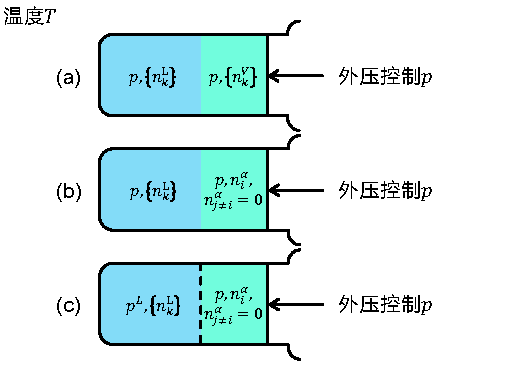
\includegraphics{../images/sol_thermodyn_typical_problems.pdf}
    \caption{恒定温度下,液体混合物的三种典型相平衡问题。(a) 气液共存,两相压强相同,且物质自由交换;(b) “非挥发溶质”相平衡问题,两相压强相同,只有组份$i$(溶剂)在两相间自由交换;(c) 半透膜问题,两相压强不同,只有组份$i$在两相间自由交换。}
    \label{fig:sol_thermodyn_typical_problems}
\end{figure}

此时我们需要把上式的化学势的具体表达式写出来,面临标准态的选择问题。留意到,标准态的选择原则中有一条“避免相变”,即体系从所选择的标准态到当前态的过程不发生相变。这在本问题当中就要求视气、液相为两个不同的状态方程所描述的体系,各状态方程均不描述该体系的气、液相变和共存行为,仅为我们分别考虑各相时使用。

如果我们分别为气、液两相选择拉乌尔定律标准态,则有
\begin{equation*}
    \mu_i^\alpha\left(T,p,\left\{n_j^\alpha\right\}\right)=\mu_i^{*,\alpha}\left(T,p\right)+RT\ln a_i^\alpha\left(T,p,\left\{n_j^\alpha\right\}\right),\quad i=1,2,\cdots,\quad \alpha=\text{V},\text{L}
\end{equation*}
其中,组份$i$纯物质在不同相态下的化学势$\mu_i^{*,\alpha}$及其在不同相态混合物中的活度$a_i^\alpha$是关于$\left(T,p,\left\{n_i^\alpha\right\}\right)$的不同的函数,源自两相各自的状态方程。把这种表达式代入相平衡条件,标准态的化学势不能被消掉。这又不符合标准态选择的原则。

纯物质$i$在给定温度下,处于气、液共存平衡态时的压强——即纯物质$i$的蒸气压$p_i^{*,\text{vap}}=p_i^{*,\text{vap}}\left(T\right)$时,由相平衡条件有
\[\mu_i^{*,\text{V}}\left(T,p_i^{*,\text{vap}}\right)=\mu_i^{*,\text{L}}\left(T,p_i^{*,\text{vap}}\right)\]
这为我们提供了一个适用于考虑混合物的气液共存问题的标准态。以这个状态为标准态,则
\begin{equation*}
    \mu_i^\alpha\left(T,p,\left\{n_j^\alpha\right\}\right)=\mu_i^{*,\alpha}\left(T,p_i^{*,\text{vap}}\right)+RT\ln\frac{f_i^\alpha\left(T,p,\left\{n_j^\alpha\right\}\right)}{f_i^{*,\alpha}\left(T,p_i^{*,\text{vap}}\right)},\quad i=1,2,\cdots,\quad\alpha=\text{V},\text{L}
\end{equation*}
代入相平衡条件后得到
\[\frac{f_i^\text{V}\left(T,p,\left\{n_j^\text{V}\right\}\right)}{f_i^{*,\text{V}}\left(T,p_i^{*,\text{vap}}\right)}=\frac{f_i^\text{L}\left(T,p,\left\{n_j^\text{L}\right\}\right)}{f_i^{*,\text{L}}\left(T,p_i^{*,\text{vap}}\right)},\quad i=1,2,\cdots\]
其中,$f_i^{*,\alpha}$是组份$i$纯物质在不同相态下的逸度,它们直接联系到组份$i$纯物质不同相态下的状态方程。

以下我们逐步往理想体系靠拢。首先如果各相是理想混合物(但气相暂未必是理想气体混合物),则上式化为
\[\ln x_i^\text{V}+\ln\frac{f_i^{*,\text{V}}\left(T,p\right)}{f_i^{*,\text{V}}\left(T,p_i^{*,\text{vap}}\right)}=\ln x_i^\text{L}+\ln\frac{f_i^{*,\text{L}}\left(T,p\right)}{f_i^{*,\text{L}}\left(T,p_i^{*,\text{vap}}\right)},\quad i=1,2,\cdots\]
其中用到了理想混合物活度系数等于1的条件。气态纯物质保持使用逸度是因为气态虽是理想混合物但不是理想气体混合物,所以至少有些组分纯物质气态不遵守理想气体状态方程。由逸度与(偏)摩尔体积的关系,有
\[\ln\frac{f_i^{*,\alpha}\left(T,p\right)}{f_i^{*,\alpha}\left(T,p_i^{*,\text{vap}}\right)}=\int_{p_i^{*,\text{vap}}}^p\frac{V_{\text{m},i}^{*,\alpha}\left(T,p^\prime\right)}{RT}\mathrm{d}p^\prime,\quad i=1,2,\cdots,\quad \alpha=\text{V},\text{L}\]
则各相均为理想混合物情况的关系式变为
\[\ln x_i^\text{V}+\int_{p_i^{*,\text{vap}}}^{p}\frac{V_{\text{m},i}^{*,\text{V}}\left(T,p^\prime\right)}{RT}\mathrm{d}p^\prime=\ln x_i^\text{L}+\int_{p_i^{*,\text{vap}}}^{p}\frac{V_{\text{m},i}^{*,\text{L}}\left(T,p^\prime\right)}{RT}\mathrm{d}p^\prime,\quad i=1,2,\cdots\]

再往理想体系靠拢一步:若某组份$i$纯物质的气态是理想气体,即
\[V_{\text{m},i}^{*,\text{V}}\left(T,p\right)=RT/p\]
则对这个组份$i$就有
\[\ln x_i^\text{V}+\ln\frac{p}{p_i^{*,\text{vap}}}=\ln x_i^\text{L}+\int_{p_i^{*,\text{vap}}}^{p}\frac{V_{\text{m},i}^{*,\text{L}}\left(T,p^\prime\right)}{RT}\mathrm{d}p^\prime \]
若各组份$i$纯物质的气态都是理想气体(即混合物体系的气态是理想气体混合物),则上式对各组份$i=1,2,\cdots$均成立。

若考虑液态的体积随压强的变化很小,则等号右边的积分也可以略掉,我们就得到
\[x_i^\text{V}p=x_i^\text{L}p_i^{*,\text{vap}},\quad i=1,2,\cdots\]
再加上气相是理想气体混合物,满足道尔顿分压定律,上式左边是组份$i$在气相中的分压$p^\text{V}_i=x_i^\text{V}p$,故上式又进一步写成
\[p_i^\text{V}=x_i^\text{L}p_i^{*,\text{vap}},\quad i=1,2,\cdots\]
这就是拉乌尔定律。

可见,拉乌尔定律包括以下假定:
\begin{itemize}
    \item 气相是理想气体混合物;
    \item 液相是理想混合物;
    \item 液相不可压缩。
\end{itemize}

我们如果不为了“消掉”而给两相选择统一的标准态,保持液相是理想混合物、气相是理想气体混合物的条件,按照各相通常的参考态选择方式,组份$i$在各相的化学势可以写成
\begin{align*}
    \mu_i^\text{V,ig}\left(T,p,\left\{n_j^\text{V}\right\}\right) & =\mu_i^\text{V,*,ig}\left(T,p^\circ\right)+RT\ln\frac{p}{p^\circ}+RT\ln x_i^\text{V}, \\
    \mu_i^\text{L,id}\left(T,p,\left\{n_j^\text{L}\right\}\right) & =\mu_i^\text{L,*,id}\left(T,p\right)+RT\ln x_i^\text{L},                              \\
    i                                                             & =1,2,\cdots
\end{align*}
代入相平衡条件后得
\[
    \mu_i^\text{L,*,id}\left(T,p\right)-\mu_i^\text{V,*,ig}\left(T,p^\circ\right)+RT\ln p^\circ+RT\ln x_i^\text{L}-RT\ln\left(x_i^\text{V}p\right)=0,\quad i=1,2,\cdots
\]
引入组份$i$的亨利系数$k_i$,满足
\[RT\ln k_i=\mu_i^\text{L,*,id}\left(T,p\right)-\mu_i^\text{V,*,ig}\left(T,p^\circ\right)+RT\ln p^\circ,\quad i=1,2,\cdots\]
则有
\[p_i^\text{V}=k_ix_i^\text{L}\]
这就是亨利定律。与拉乌尔定律相比较可见,拉乌尔定律中的比例系数是组份$i$纯物质在温度$T$下的蒸气压$p_i^{*,\text{vap}}=p_i^{*,\text{vap}}\left(T\right)$,仅为温度的函数;而亨利定律中的比例系数$k_i=k_i\left(T,p\right)$是温度和压强的函数,且其数值依赖所选定的参考压强值$p^\circ$。这个差别是推导亨利定律没有采用推导拉乌尔定律时使用的“液相不可压缩”的等效后果。

值得注意的是,混合物在各相内的各组份摩尔分数$x_i$满足$\sum_ix_i\equiv 1$的约束。由于这一约束,我们以下将推出,对于液相是理想混合物、气相是理想气体混合物的体系,如果确定了$j\neq i$的亨利系数,则剩下的这个组份$i$的气液相分配也就已被确定。由
\[x_j^\text{V}p=k_jx_j^\text{L},\quad j\neq i\]
和各组份的相平衡条件
\[\mu_k^\text{L}=\mu_k^\text{V}\Leftrightarrow \mathrm{d}\mu_k^\text{L}=\mathrm{d}\mu_k^\text{V},\quad k=1,2,\cdots\]
以及恒温恒压下的吉布斯--杜亥姆方程有(只应用于液相)
\[
    n_i^\text{L}\mathrm{d}\mu_i^\text{L}+\sum_{j\neq i}n_j\text{L}\mathrm{d}\mu_j^\text{L}=0\Leftrightarrow n_i^\text{L}\mathrm{d}\ln\left(x_i^\text{V}p\right)+\sum_{j\neq i}n_j^\text{L}d\ln\left(k_jx_j^\beta\right)
\]
而
\begin{align*}
    \sum_{j\neq i}n_j^\text{L}\mathrm{d}\ln\left(k_j x_j^\text{L}\right) & =\sum_{j\neq i}\frac{n_j}{x_j^\text{L}}\mathrm{d}x_j^\text{L} \\
                                                                         & =n\sum_{j\neq i}\mathrm{d}x_j^\text{V}                        \\
                                                                         & =-n\mathrm{d}x_i^\text{L}
\end{align*}
其中运用了$k_j$只依赖$T$、$p$的条件(故在恒温恒压下的微分按常数处理),以及$x_i^\text{L}=1-\sum_{j\neq i}\mathrm{d}x_j^\text{L}$。
因此液相的吉布斯--杜亥姆方程就变成以下微分方程:
\[\frac{\mathrm{d}x_i^\text{L}}{x_i^\text{L}}=\mathrm{d}\ln\left(x_i^\text{V}p\right)\]
利用$x_i^\text{L}=1$时$x_i^\text{V}=1$的条件解上列方程得
\[x_i^\text{L}p\left(x_i^\text{V}= 1\right)=p x_i^\text{L}\Leftrightarrow x_i^\text{L}p_i^{*,\text{vap}}=p^\text{V}_i\]
即组份$i$满足拉乌尔定律。与之前得到的所有组份满足拉乌尔定律相比较,这里的结论是仅一个组份满足拉乌尔定律,其余组份满足亨利定律,这是不需要依靠“液相不可压缩”条件,仅基于液相是理想混合物、气相是理想气体混合物就能得到的结论。如果把组份$j\neq i$称作“溶质”,则组份$i$就是溶剂,于是也就得到通常《物理化学》教科书中,所谓“理想溶液”\footnote{“溶液”一词专用于讨论混合物时区分溶质和溶剂的情况。除此之外,若不再加其他说明,那么“理想溶液”就应就等价于“理想混合物”。但既然对“理想溶液”的溶质溶剂遵守这两个定律的陈述,那似乎又认为“理想溶液”在气液共存时气态总是理想气体混合物,而不仅只是处于气态的理想混合物。这是普通的《物理化学》课本不够严谨的地方。}的溶剂满足拉乌尔定律(而无需要求其液相不可压缩)、溶质满足亨利定律的结论。

\subsection{“非挥发溶质”问题}
有一类问题是液态混合物与其某一组份纯物质的另一相态之间在定温下的相平衡问题(如图\ref{fig:sol_thermodyn_typical_problems}(b)所示)。这类问题的相平衡条件是
\begin{equation}\label{eq:II.5_phase_eq_non_volatile}
    \mu_i^\text{L}\left(T,p,\left\{n_k^\text{L}\right\}\right)=\mu_i^{\alpha,*}\left(T,p\right),\quad n_{j\neq i}^\alpha=0,\quad \alpha=\text{V},\text{L或S}
\end{equation}

如果$\alpha$相是气相($\alpha=\text{V}$),视组份$j\neq i$为“溶质”,就可以称其为“非挥发”的溶质。只有“溶剂”组份$i$有气液共存的行为。

如果$\alpha$相是固相($\alpha=\text{S}$),则类似组份$i$在一个溶液中“析出”其晶体(或称“重结晶”)。

如果$\alpha$相是液相($\alpha=\text{L}$),则类似该液体混合物发生了“分层”,且有一相几乎没有其他组份$j\neq i$的奇怪情况。

尽管第三种情况很少见,但无论$\alpha$相是什么物态,以下讨论的热力学结论是普适的。应用时只需按以下几种情况作相应的解度就可以了。假定体系在当前$\left(T,p,\left\{n_j\right\}\right)$取值下处于如式\eqref{eq:II.5_phase_eq_non_volatile}所表达的稳定的平衡态,那么:
\begin{itemize}
    \item $n_i$是组份$i$在$T$、$p$下,其余组成为$\left\{n_{j\neq i}\right\}$时的溶解度;
    \item $T$是液相混合物在该$p$下,组成为$\left\{n_j\right\}$时的的相变点。例如当$\alpha=\text{V}$时是液相混合物在该条件下的沸点;当$\alpha=\text{S}$时是组份$i$从该条件下的液相混合物析出的凝固点;
    \item $p$是组份$i$在$T$下,与组成为$\left\{n_j\right\}$的液相混合物共存时的饱和蒸气压。
\end{itemize}

因此由式\eqref{eq:II.5_phase_eq_non_volatile}出发的以下分析,将使我们获得上述这些性质的变化规律。由式\eqref{eq:II.5_phase_eq_non_volatile},在当前状态点附近的微变化将满足
\begin{align*}
                    & \mathrm{d}\mu_i^\text{L}\left(T,p,\left\{n_i^\text{L}\right\}\right)=\mathrm{d}\mu_i^{\alpha,*}\left(T,p\right)                                                                                                                                                                             \\
    \Leftrightarrow & -S_i^\text{L}\mathrm{d}T+V_i^\text{L}\mathrm{d}p+\sum_j\left.\frac{\partial \mu_i^\text{L}}{\partial n_j^\text{L}}\right|_{T,p,\left\{n_{k\neq j}\right\}}\mathrm{d}n_j^\text{L}=-S_{\text{m},i}^{\alpha,*}\mathrm{d}T+V_{\text{m},i}^{\alpha,*}\mathrm{d}p,\quad\alpha=\text{V},\text{L或S}
\end{align*}
由于液相只有组份$i$的摩尔数发生变化(与气相交流),而其他组份$j\neq i$都不变化,因此上式变为
\begin{align*}
                    & -S_i^\text{L}\mathrm{d}T+V_i^\text{L}\mathrm{d}p+\left.\frac{\partial\mu_i^\text{L}}{\partial n_i^\text{L}}\right|_{T,p}\mathrm{d}n_i^\text{L}=-S_{\text{m},i}^{\alpha,*}\mathrm{d}T+V_{\text{m},i}^{\alpha,*}\mathrm{d}p                                                                                                                                                               \\
    \Leftrightarrow & -\left(S_i^\text{L}-S_{\text{m},i}^{\alpha,*}\right)\mathrm{d}T+\left(V_i^\text{L}-V_{\text{m},i}^{\alpha,*}\right)\mathrm{d}p+\left.\frac{\partial \mu_i^\text{L}}{\partial n_i^\text{L}}\right|_{T,p}\mathrm{d}n_i^\text{L}=0                                                                                                                                                         \\
    \Leftrightarrow & \mathrm{d}n_i^\text{L}=-\frac{V_i^\text{L}-V_{\text{m},i}^{\alpha,*}}{\left(\partial\mu_i^\text{L}/\partial n_i^\text{L}\right)_{T,p}}\mathrm{d}p+\frac{S_i^\text{L}-S_{\text{m},i}^{\alpha,*}}{\left(\partial\mu_i^\text{L}/\partial n_i^\text{L}\right)_{T,p}} \mathrm{d}T                                                                                                            \\
    \Leftrightarrow & \left.\frac{\partial n_i^\text{L}}{\partial p}\right|_{T}=-\frac{V_i^\text{L}-V_{\text{m},i}^{\alpha,*}}{\left(\partial\mu_i^\text{L}/\partial n_i^\text{L}\right)_{T,p}},\quad\left.\frac{\partial n_i^\text{L}}{\partial T}\right|_{p}=\frac{S_i^\text{L}-S_{\text{m},i}^{\alpha,*}}{\left(\partial\mu_i^\text{L}/\partial n_i^\text{L}\right)_{T,p}},\quad\alpha=\text{V},\text{L或S}
\end{align*}

在式\eqref{eq:II.5_phase_eq_non_volatile}成立的条件下,由偏摩尔热力学函数之间的关系,又有
\[H_i^\text{L}-TS_i^\text{L}=H_{\text{m},i}^{\alpha,*}-TS_{\text{m},i}^{\alpha,*}\Leftrightarrow H_i^\text{L}-H_{\text{m},i}^{\alpha,*}=T\left(S_i^\text{L}-S_{\text{m},i}^{\alpha,*}\right)\]
故上面得到的两个偏导数又可表示为:
\[\left.\frac{\partial n_i^\text{L}}{\partial p}\right|_{T}=\frac{V_{\text{m},i}^{\alpha,*}-V_i^\text{L}}{\left(\partial \mu_i^\text{L}/\partial n_i^\text{L}\right)_{T,p}},\quad\left.\frac{\partial n_i^\text{L}}{\partial T}\right|_{p}=-\frac{\lambda_i}{T}\frac{1}{\left(\partial\mu_i^\text{L}/\partial n_i^\text{L}\right)_{T,p}}\]
其中$\lambda_i\equiv H_{\text{m},i}^{\alpha,*}-H_i^\text{L}$。另外,由《物理化学》附录\S I.3的式(7)可得到
\[\left.\frac{\partial p}{\partial T}\right|_{n_i^\text{L}}=\frac{\lambda_i}{T\left(V_{\text{m},i}^{\alpha,*}-V_i^\text{L}\right)}\]
注意上列式子均只在使式\eqref{eq:II.5_phase_eq_non_volatile}成立的条件下成立。

由平衡态的稳定性判据,这些偏导数表达式中的$\partial\mu_i^\text{L}/\partial n_i^\text{L}>0$。因此它们的符号由$\lambda_i$或$V_i^{\alpha,*}-V_i^\text{L}$的符号决定。

$\lambda_i$是每摩尔组份$i$从纯物质$\alpha$状态变为置身于同温同压下相应组成$\left\{n_j\right\}$的液相状态的焓变。它与两状态中组份$i$分子处于的分子间作用力强弱差异有关。分子间力增大,这个过程的焓变为负。换个角度也可以说$\lambda_i>0$表示溶解时放热,反之亦然。

$V_{\text{m},i}^{\alpha,*}-V_i^\text{L}$是组份$i$纯物质在$\alpha$相的(偏)摩尔体积与其处于同温同压下其在组成为$\left\{n_j^\text{L}\right\}$的液相混合物时的偏摩尔体积之差。一般来说,气、液、固态物质,摩尔体积依次大幅减小,这个差异比同相态不同组成间的差异大。

现在考虑偏微分$\left(\partial n_i^\text{L}/\partial T\right)_{p}$。如果$\alpha$相是气态,那么一般从气态到液态分子间力增大,所以$\lambda_i>0$,此时温度升高,组份$i$在液相的溶解度降低。若$\alpha$是固相,由于一般从固态到液态分子间力减小,所以$\lambda_i<0$,此时温度升高时组份$i$在液相的溶解度增加。若$\alpha$是液相,$\lambda_i$没有通常的情况可以讨论。再考虑该偏微分的倒数$\left(\partial T/\partial n_i^\text{L}\right)_p$,当$\alpha$相是气相时,沸点随组份$i$在液相浓度减小而增加。若视组份$i$为“溶剂”,则可说溶质浓度增加将使溶液的沸点增加。若$\alpha$是固相,组份$i$的凝固点随其在液相中浓度的减小而降低。若视组份$i$为“溶剂”,则溶质浓度增加将使溶剂凝固点降低。以上这些性质均在《物理化学》\S4.8以“溶剂服从拉乌尔定律、溶质服从亨利定律”的情况推导过了。以下我们从一般混合物出发,在“稀溶液极限”得出相应的表达式。

之前得到的一个偏导数$\left(\partial T/\partial n_i^\text{L}\right)_{p}$的倒数,可解读成等温条件下混合物的L-$\alpha$共存温度$T=T_\text{c}$随组成$n_i^\text{L}$的变化率
\begin{equation}\label{eq:II.5_phase_coexist_temperature_partial_derivative}
    \left.\frac{\partial T_\text{c}}{\partial n_i^\text{L}}\right|_{p}=-\left.\frac{\partial \mu_i^\text{L}}{\partial n_i^\text{L}}\right|_{T_\text{c},p}\frac{T_\text{c}}{\lambda_i}
\end{equation}
视混合物的L-$\alpha$共存温度是组份$i$在混合物中的摩尔分数$x_i^\text{L}$的函数,$T_\text{c}=T_\text{c}\left(x_i^\text{L}\right)$,则它在$x_i^\text{L}$附近的展开式为
\[T_\text{c}\left(x_i^\text{L}\right)=T_{i,\text{c}}^*+\left.\frac{\partial T_\text{c}}{\partial x_i^\text{L}}\right|_{p,x_i^\text{L}=1}\left(x_i^\text{L}-1\right)+o\left[\left(x_i^\text{L}-1\right)^2\right]\]
其中$T_{i,\text{c}}^*\equiv T_\text{c}\left(1\right)$是纯份$i$液态纯物质在同压强$p$下的L-$\alpha$共存温度温度,而
\[\frac{\partial T_\text{c}}{\partial x_i^\text{L}}=\frac{\partial T_\text{c}}{\partial n_i^\text{L}}\frac{\partial n_i^\text{L}}{\partial x_i^\text{L}}\]
可见,利用式\eqref{eq:II.5_phase_coexist_temperature_partial_derivative},可以表出在$x_i^\text{L}$很接近1时的L-$\alpha$共存温度表达式。这里还需要推导的是导数$\partial n_i^\text{L}/\partial x_i^\text{L}$。由于L相混合物除组份$i$之外的剩余组份的摩尔数$n^\text{L}-n_i^\text{L}$保持恒定,令$C\equiv n^\text{L}-n_i^\text{L}$,则$n_i^\text{L}$与$x_i^\text{L}$的关系可表示为
\[n_i^\text{L}=\frac{Cx_i^\text{L}}{1-x_i^\text{L}}\]
进而
\[\frac{\partial n_i^\text{L}}{\partial x_i^\text{L}}=\frac{C}{\left(1-x_i^\text{L}\right)^2}=\frac{n^\text{L}}{1-x_i^\text{L}}\]
进而
\[\frac{\partial T_\text{c}}{\partial x_i^\text{L}}=-\frac{T_\text{c}}{\lambda_i}\frac{\partial\mu_i^\text{L}}{\partial n_i^\text{L}}\frac{n^\text{L}}{1-x_i^\text{L}}\]
把式\eqref{eq:II.4_Raoult_standard_state_activity}在$T=T_\text{c}$时的形式代入上式,得到
\[\left.\frac{\partial T_\text{c}}{\partial x_i^\text{L}}\right|_{p,x_i^\text{L}=1}=-\frac{R\left(T_{i,\text{c}}^*\right)^2}{\Delta_\text{c}H_{\text{m},i}^*}\]
其中用到了$x_i^\text{L}=1$时$\partial \gamma_i^\text{L}/\partial n_i^\text{L}=0$,并且记
\[\Delta_\text{c}H_{\text{m},i}^*\equiv\lambda_i\left(x_i^\text{L}=1\right)=H_{\text{m},i}^{\alpha,*}-H_{\text{m},i}^{\text{L},*}\]
为组份$i$纯物质的L-$\alpha$相变焓。代入$T_\text{c}\left(x_i^\text{L}\right)$的展开式可得,液体理想混合物在$x_i^\text{L}$很接近1时
\[\Delta T_\text{c}\approx\frac{R\left(T_{i,\text{c}}^*\right)^2}{\Delta_\text{c}H_{\text{m},i}^*}\left(1-x_i^\text{L}\right)\]
若视组份$i$为溶剂,省去上标L,得到
\[\Delta T_\text{c}\approx \frac{R\left(T_{i,\text{c}}^*\right)^2}{\Delta_\text{c}H_{\text{m},i}^*}x_\text{B}\]
其中$x_\text{B}\equiv 1-\sum_j x_{j\neq i}$是溶质的摩尔分数。

若$\alpha$相是气相,则纯溶剂的摩尔蒸发焓$\Delta_\text{vap}H_{\text{m},i}^*=\Delta_\text{c}H_{\text{m},i}^*$,$\Delta T_\text{b}=\Delta T_\text{c}$,上式就是“沸点升高”的公式(《物理化学》式(4.67));若$\alpha$相是固相,则组份$i$纯物质的摩尔熔化焓$\Delta_\text{fus}H_{\text{m},i}^*=-\Delta_\text{c}H_{\text{m},i}^*$,$\Delta T_\text{f}=-\Delta T_\text{c}$,上式就是“凝固点降低”的公式(《物理化学》式(4.64))。

现在考虑偏微分$\left(\partial n_i^\text{L}/\partial p\right)_T$。无论$\alpha$相是什么相态,我们可以统一地说,加压将使组份$i$往两相中偏摩尔体积更小的相跑。再考虑该偏微分的倒数$\left(\partial p/\partial n_i^\text{L}\right)_T$,与它比较相关的实际情况是$\alpha$为气相的情况。则在温度不变时,当液相中组份$i$减小,饱和蒸气压降低。这时视组分$i$为“溶剂”,则可说溶质浓度增加将使溶液的饱和蒸气压降低。

最后一个偏微分$\left(\partial p/\partial T\right)_{n_i^\text{L}}$是液相混合物体系的克拉佩龙--克劳修斯方程。《物理化学》\S6.4的式(6.12)是这个方程的纯物质版。

\subsection{半透膜问题}
半透膜问题中,也分两相,其中一相是液态混合物,另一相是同温下某组份$i$的纯物质,但压强与液态混合物相不同(如图\ref{fig:sol_thermodyn_typical_problems}(c)所示)。这要依靠半透膜来实现。它是隔开两相的一个界面,但位置和形状是固定的。在大部分问题中,半透膜通常是导热的,允许两边的分体系之间达到热平衡。但由于它是刚的,因此能承担它两侧存在的压差。半透膜最重要的特点是,它两侧的压强之间并非独立,而是通过组分的部分透过性而相互关联的。所以可以说这种壁还允许部分物质交换。我们将推导发现,半透膜左右两相的压差——即渗透压——与可透过组份摩尔数在两相的分配有关。

具体地,设半透膜左侧是液态混合物相,压强为$p^\text{L}$;右侧为组份$i$组物质相,压强为$p$,物态不重要,故记为$\alpha$相。我们不妨假定半透膜右侧与环境外压$p$达到力学平衡,即$\alpha$相的压强$p$保持恒定。化学平衡条件
\[\mu_i^\text{L}\left(T,p^\text{L},\left\{n_j^\text{L}\right\}\right)=\mu_i^{\alpha,*}\left(T,p\right)\]
两边全微分($\mathrm{d}n_{j\neq i}^\text{L}=0,\mathrm{d}T=0,\mathrm{d}p=0$)得到
\[V_i^\text{L}\mathrm{d}p^\text{L}+\frac{\partial \mu_i^\text{L}}{\partial n_i^\text{L}}\mathrm{d}n_i^\text{L}=0\]
而由平衡态稳定性条件,$\partial\mu_i^\text{L}/\partial n_i^\text{L}>0$,故上式表明,当可透过组份$i$减小时,液体混合物相的压强增加。若视组份$i$为溶剂,并记$\Pi\eqdef p^\text{L}-p$为液体混合物的渗透压,则可以说,当溶质浓度增加时,溶液的渗透压相应增加,增加率是溶剂在溶液中的偏摩尔体积$V_i^\text{L}$。注意以上等式是在定温定压下两相体系达到稳定平衡态时成立。我们可以写下定温定压下液体混合物的渗透压随可透过组份在混合物中的浓度的变化率,即偏导数
\begin{equation}\label{eq:II.5_osmotic_pressure_partial_derivative}
    \frac{\partial\Pi}{\partial n_i^\text{L}}=\frac{\partial p^\text{L}}{\partial n_i^\text{L}}=-\frac{1}{V_i^\text{L}}\frac{\partial\mu_i^\text{L}}{\partial n_i^\text{L}}
\end{equation}

以下推导混合物在极稀条件下的范托夫定律。恒温、恒外压$p$下,渗透压可表示组份$i$在混合物相中的摩尔分数$x_i^\text{L}$的函数,其在$x_i^\text{L}=1$附近的展开式是
\[\Pi\left(x_i^\text{L}\right)=\Pi\left(1\right)+\left.\frac{\partial\Pi}{\partial x_i^\text{L}}\right|_{x_i^\text{L}=1}\left(x_i^\text{L}-1\right)+o\left[\left(x_i^\text{L}-1\right)^2\right]\]
其中$\Pi\left(1\right)=0$,而
\[\frac{\partial \Pi}{\partial x_i^\text{L}}=\frac{\partial\Pi}{\partial n_i^\text{L}}\frac{\partial n_i^\text{L}}{\partial x_i^\text{L}}\]
可见,利用式\eqref{eq:II.5_osmotic_pressure_partial_derivative},可以表出在$x_i^\text{L}$很接近1时的渗透压表达式。这里所需要的偏导数$\partial n_i^\text{L}/\partial x_i^\text{L}$之前已经推导过了。我们直接可以得到
\[\left.\frac{\partial \Pi}{\partial x_i^\text{L}}\right|_{x_i^\text{L}=1}=-\frac{RT}{V_i^\text{L,*}}\]
再代入$\Pi\left(x_i^\text{L}\right)$的展开式可得,液态理想混合物在$x_i^\text{L}$很接近1时
\[\Pi\approx\frac{RT}{V_i^\text{L,*}}\left(1-x_i^\text{L}\right)\]
若视组份$i$为溶剂,且在$x_i^\text{L}\rightarrow 1$时
\[V_i^\text{L,*}=V^\text{L}/n_i^\text{L}\approx V^\text{L}/n^\text{L}\]
省去上标L,有
\[\Pi V\approx RTn_\text{B}\]
其中$n_\text{B}\equiv\sum_{j\neq i}n_j$是溶质的物质的量。该式就是《物理化学》\S4.9式(4.73)的范托夫定律(van 't Hoff law)。我们留意到,范托夫定律仅是稀溶液极限下的近似行为。若不在稀的极限,展开式的二次方项不可忽略,上式因含有第二位力系数而依赖体系的化学属性,不再是“依数性”。在《物理化学》中的\S4.9“理想稀溶液的依数性”之下介绍的式(4.76)、(4.77)超出了该节的主题。
\end{document}